\documentclass[a4paper, 12pt, oneside]{report}

\usepackage[top=2.5cm,bottom=2.5cm,left=2.5cm,right=2.5cm]{geometry}
%%%%%%%%%%%%%%%%%%%%%%%%%%%%%%%%%%%%%%%%%%%%%%%%%%%%%%%%%%%%%%%%%%%%%%%%%%%%%%%%%%%%%%%%%%%%%%%
%%% A choisir l'un des deux packages suivants selon si vous êtes sous Linux ou bien Windows %%%
\usepackage[utf8]{inputenc} % linux
%\usepackage[latin1]{inputenc} % windows
%%%%%%%%%%%%%%%%%%%%%%%%%%%%%%%%%%%%%%%%%%%%%%%%%%%%%%%%%%%%%%%%%%%%%%%%%%%%%%%%%%%%%%%%%%%%%%%
\usepackage[frenchb]{babel}
%\usepackage[english]{babel}
%\usepackage[english,francais]{babel}
\usepackage[pdftex]{graphicx}
%\usepackage{epstopdf} 
\usepackage{graphics}
\usepackage{url}
\usepackage{fancyhdr} 
% Entête/ Pieds de page:  \pagestyle{empty}: aucune en-tête et aucun pied de page ne seront affichés.
% \pagestyle{plain}: seul le numéro de page est affiché au centre du pied de page.
% \pagestyle{headings}: les en-têtes et les pieds de page sont définis automatiquement selon la classe de document utilisée.
\usepackage{color}
%-----------------------------
\usepackage{subfig}
%\usepackage{multirow}
\usepackage{array,multirow}
%------------------------------------
%\usepackage{amsmath} Remarque: ce package est utile si vous souhaitez écrire des symboles et des formules mathématiques. 
%\usepackage{url}
\linespread{1.5}

\pagestyle{fancy}
\usepackage[Lenny]{fncychap}
\begin{document}
\begin{titlepage}

\begin{figure}[htbp]
 \hbox{
     
\includegraphics[width=40px]{logo.png}
     \hspace*{12.5cm}
     
\includegraphics[width=40px]{logo.png}
  }
\end{figure}

\vspace {-1.8cm}

\begin{center}
%%%%%% En-tete
{\bf R\'{e}publique Alg\'{e}rienne D\'emocratique et Populaire\\
Minist\`{e}re de l'Enseignement Sup\'{e}rieur et de la
Recherche Scientifique} \vspace{0.2cm}\\

{\bf {\large Universit\'{e} AMO de Bouira}}\\

{\bf Facult\'{e} des Sciences et des Sciences Appliquées} \\

{ \textbf{D\'epartement d'Informatique}}\\ \vspace{0.8cm}
%%%%%%%%%%%%%%%%%%%%%%%%%%%%%%%%%%%%%%%%%%%%%%%%%%%%%%%%%
\Huge{\textbf{Mémoire de Licence}} \\ \Large{\textbf{en Informatique}} \\\vspace{0.3cm}
\large{\emph{\textbf{Spécialité:} Votre spécialité}}\\ \vspace{0.8cm}
\huge{\textbf{Thème}}\\ %\vspace{0.3cm}
\noindent\rule{\textwidth}{1mm}
\Large{\textbf{Titre de votre projet}}
\noindent\rule{\textwidth}{1mm}
\end{center}
\vspace{0.3cm}
%%%%%%%%%%%%%%%%%%%%%%%%%%%%%%%%%%%%%%%%%%%%%%%%%%%%%%%%
\begin{tabular}{ p{9cm}  p{6cm} }
\textbf{Encadré par} & \textbf{Réalisé par} \\
\begin{itemize}
	\item \textsc{Nom} Encadreur
\end{itemize}
&
\begin{itemize}
	\item \textsc{Nom} Étudiant 1
	\item \textsc{Nom} Étudiant 2
\end{itemize}
\\
\end{tabular}
\vspace{4.5cm}
\begin{center}
2015/2016
\end{center}

\end{titlepage}
\pagestyle{empty}
%%%% \addcontentsline{toc}{chapter}{Remerciements}
% \chapter*{Remerciements} 
%
\begin{center}
\huge{\emph{Acknowledgement}}
\end{center}

\vspace{1cm}

\paragraph{}
First of all, let’s thank Allah who has been giving us some mercies and blessing so that we have done this project without any troubles at all. Secondly, may prayers and peace be upon our Prophet Muhammad who has guided us from the darkness to the lightness in the world as well as in the next world.\\\\
\indent Thank you our supervisor, Dr. TAHA ZERROUKI, for your patience, guidance, and support. We have benefited greatly from your wealth of knowledge and meticulous editing. We are grateful that you took us on as the team of this project and continued to have faith in us over the years.\\\\
\indent Thank you our colleagues involved directly or indirectly with encouraging words and thoughtful, detailed feedback have been very important to us.\\\\
\indent Thank you to everyone, who so generously took time out of their schedules to review our project and gave us constractive feedback.\\\\
\indent Thank you to our parents, for your endless support. They have always stood behind us, and this was no exception. Thank you for all of your love and for always reminding us of the end goal.\\

%%%\newpage
%%%\begin{center}
\Huge{\emph{Dedications}}
\end{center}

\vspace{1cm}

First, I would like to dedicate this work to the most important people in my life, to the ones who supported me and guided me diligently throughout this work and throughout my whole life, to my mother and my father. I also dedicate this work to my brother and sisters, and of course to my team, Farouk and Mohammed, with whom I was able to accomplish this work.


\vspace{3cm}
\begin{flushright}
	\textit{Grine Lyes}
\end{flushright}
%%%\newpage
%%%\newpage
%%%\begin{center}
\Huge{\emph{Dédicaces}}
\end{center}

\vspace{1cm}

Lorem ipsum ...

\vspace{3cm}
\begin{flushright}
	\textit{Nom étudiant 2.}
\end{flushright}
\newpage
%%%\begin{figure*}[ht]
	\centering
	\label{}
\includegraphics[scale=0.8]{img/resume.pdf} 
                
\end{figure*}

\section*{Abstract}
\paragraph{}Interactive courses help students better understand their lessons through interactive quizzes and examples that test their knowledge and help them better understand the lessons.
\\We have noticed that the subject of the computer architecture lacks such applications, especially since most students have the technological means that allow it, such as mobile phones and computers, especially since they do today an integral part of social life.
That is what inspired us to find and realize the idea of the project.
\paragraph{}


\section*{Résumé}

\paragraph{}Les leçons interactives aident les élèves à mieux comprendre leurs leçons grâce à des tests interactifs et des exemples qui testent leurs connaissances et les aident à mieux comprendre les leçons.
\\ Nous avons remarqué que le sujet de la structure des machines manque de telles applications, d'autant plus que la plupart des étudiants possèdent les moyens technologiques qui le permettent, tels que les téléphones portables et les ordinateurs, d'autant plus qu'ils font aujourd'hui partie intégrante de la vie sociale.
Ce qui nous a inspiré pour trouver et concrétiser l'idée du projet.



\newpage
\pagestyle{fancy}
\pagenumbering{roman}
\lhead{}
\rhead{\textit{Table des matières}}
\addcontentsline{toc}{chapter}{Table des matières}
\tableofcontents{}
\newpage
\lhead{}
\rhead{\textit{Table des figures}}
\addcontentsline{toc}{chapter}{Table des figures}
\listoffigures{}
\newpage
\newpage
\lhead{}
\rhead{\textit{Liste des tableaux}}
\addcontentsline{toc}{chapter}{Liste des tableaux}
\listoftables
\newpage
\chapter*{Abreviations list}
\addcontentsline{toc}{chapter}{Abreviations list}
\lhead{}
\rhead{\textit{Abreviations list}}

\begin{tabular}{ll}
RWD & Responsive Web Design \\
IC  & Interactive Course \\
MI  & Math and Computer Science \\
AMO & AKLI MOHAND OULHADJ university \\
STRM & Computer Architecture or Structure Machine\\
\end{tabular}
\newpage
\pagenumbering{arabic}
\chapter*{General Introduction}
\addcontentsline{toc}{chapter}{General Introduction}
\lhead{}
\rhead{\textit{General Introduction}}

\paragraph{}
As new students at the university, we noticed the difficulty of adapting to the new system of study and the linguistic discrepancy, in addition to the difficulty of communicating and interacting directly with professors.

\paragraph{}
In the machine structure lessons, we noticed the possibility of developing and embodying its lessons into applications that contain interactive lessons and examples in order to help students gain a deeper understanding of the lessons.


\paragraph{}
Computer architecture is a science or a set of rules stating how computer software and hardware are joined together and interact to make a computer work. It not only deter-mines how the computer works but also of which technologies the computer is capable.\cite{Computer-Architecture-saylor-academy}


\paragraph{}
In our case and as distant as our search goes there are no as of now existing solutions(neither apps nor websites), but there exists a few tools, websites and mobile apps that are to some degree related to our extend.

\paragraph{}
Our manuscript is structured in three chapters:\\\\
First, chapter will talk about the general dedefinitions of computer architecture, role, and problem in distributing them, and we will mention examples of the existing applications.
\\Second chapter, In this chapter we will present the conceptual solution for our application, and introduce a detailed demo of our app to explain its basic functions and structure. But before that, we will present Modelling tool used: UML.
\\Third chapter, we will talk about the environment (Work and Software) and about the will use programming languages and presentation of graphical interfaces. 

\chapter{Preliminary study}
\lhead{\textit{Chapitre \thechapter}}
\rhead{\textit{Premier chapitre}}

\section{Introduction}
Lorem ipsum dolor sit amet, consectetur adipisicing elit, sed do eiusmod
tempor incididunt ut labore et dolore magna aliqua. Ut enim ad minim veniam


\section{General Definitions}
\subsection{Website}
A website is a collection of publicly accessible, interlinked Web pages that share 
a single domain name. Websites can be created and maintained by an individual, group, 
business or organization to serve a variety of purposes.\cite{Techopedia2011-zo}

\subsection{Responsive Web Design}
Responsive web design (RWD) is a web development approach that creates dynamic 
changes to the appearance of a website, depending on the screen size and orientation of 
the device being used to view it. RWD is one approach to the problem of designing for 
the multitude of devices available to customers, ranging from tiny phones to huge desktop monitors.\cite{noauthor_undated-an}

\subsection{Interactive Course}
The term "Interactive Course" (IC) typically describes material of an educational nature 
delivered in a format which allows the user to directly impact the materials content, pace, and out-come.
An example of such material would be a computer based presentation requiring a user to select the correct 
answer to a give question before proceeding to the next topic.
These types of courses are almost always computer based and most likely to be delivered to the user thru the internet. 
Due to their convenient delivery, availability and almost endless subject matter, 
interactive courses have become a major tool for those seeking to provide as well as those seeking to obtain education, 
training or certification in a given area of study.\\
With growing access and availability to computers and the internet, many schools, universities, 
businesses and government agencies are turning to IC's to train and educate their students and staff.\cite{noauthor_undated-dt}

\subsection{Computer Architecture}
\subsubsection{In general}
Computer architecture is a science or a set of rules stating how computer software and hardware are 
joined together and interact to make a computer work. It not only determines how the computer works 
but also of which technologies the computer is capable.\cite{Pam2018-so}
\subsubsection{In our case}
Computer architecture or better known as "Structure Machine"(STRM) is a course for first-year 
students in the Math and Computer Science department (MI) 
of the university bouira AMO. and also in all the MI departments in Algeria universities.\\ \\
\indent Computer architecture (STRM) has a coefficient of 3 and a credit of 5, which makes it one of the more fundamental courses.

\section{Study of the existing}
We did go over the definition of computer architecture in a general sense and in our context of study(STRM),
so in this part we will go more in-depth about the structure of the computer architecture(STRM) course (see Figure~\ref{fig:STRM}), 

\subsection{Structure of the computer architecture course}

\begin{figure} [h!]%[htbp]
 	\vspace*{13pt}
 	\subfloat{\label{}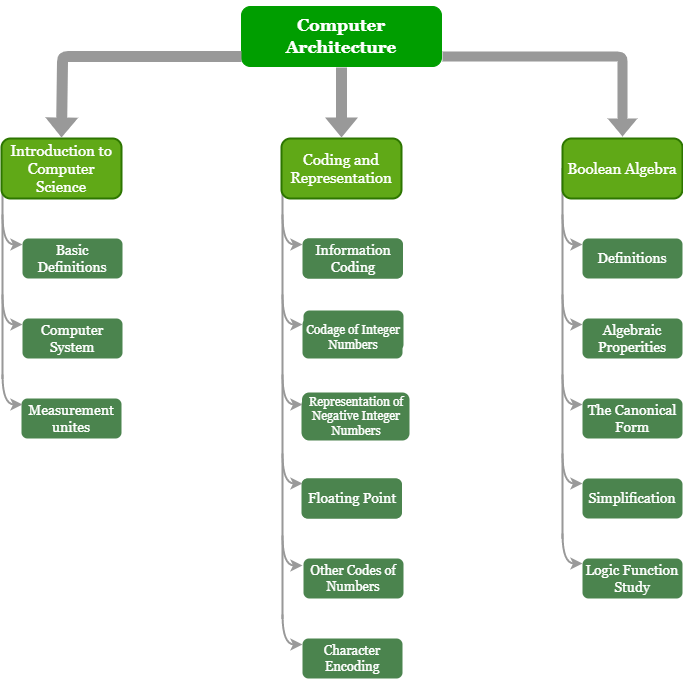
\includegraphics[scale=0.63]{img/STRM.png}} 
 	\vspace*{13pt}               
 	\caption{Structure of STRM} 
 	\label{fig:STRM}
 \end{figure} 


 \section{Analysis of existing applications}
 In this presentation ,we will talk about applications, books and similar resources about computer science, 
 where we will discuss its most important characteristics and advantages.
 There are many applications similar to our topic, but they do not contain all computer science topics.
 As for books and websites, there are many that include all computer science lessons, but they do not 
 contain the practical aspect that we will work on.
 
 \subsection{STRM 1 Book Taha Zerrouki}
 The book "The Structure of the Machine" is a book of lessons and solved exercises, intended for first-year students of mathematics and  Computer Science in 
 Algerian universities.\cite{STRM-1-Book-Taha-Zerrouki}
 It contains in this part the lessons of the first semester:
 • Elementary concepts in informatics.
 • Encoding and representing information.
 • Introduction to Boolean Algebra.
 The book contains a large number of exercises divided according to chapters, a large part of it is solved, as well as a special section for continuous assessment examinations with
 Correction, and another section for exams.
 This book comes as a result of the experience that Dr Taha gained in teaching at the University of Bouira for many years in the Department of Computer Science.
 The book is also bilingual, with lessons in French and translated into Arabic, in order to help new students who suffer from a language barrier in their college start.
 Author: Dr. Taha Zerrouki
 \subsubsection{About the author}
 Dr. Taha Zerrougui, Professor at the University of Bouira in the Department of Computer Science, Graduated from the National High School of Computers, Free Open Software Developer
 The source is exclusively in Arabic. 
 Interested in:
 • Automatic Natural Language Processing
 • open source
 Teach courses in:
 • Machine architecture and computer architecture.
 • Project management programs.
 • programming languages.
 
 \subsection{STRM Tests}
 Dr.Taha built this app to generate and create random tests for Stucture Machine 1- first Year MI, Mathematiques and Informatiques
  in Algerian universities.\cite{STRM-Tests}
 
 What this app contains:
 • Generate checks and questions with solutions
 
 • Supports the following classes:
 
 - Enumeration systems.
 - Representation of natural and real numbers and letters.
 - Encoding information.
 - Boolean algebra.
 
 • Generate answers:
 
 - Possibility to draw a logical function diagram.
 - Generate Karnoff tables.
 - Generating graphic solutions to Karnoff's table.
 
 • Generate duplicate forms of questions for easier typing.
 
 • Random generation of questions.
 
 \subsection{Computer Architecture from saylor academy}
 Saylor Academy is a nonprofit initiative working since 2008 to offer free and open online courses to all who want to learn.
  We offer nearly 100 full-length courses at the college and professional levels, each of which is available right now .
 Modern computer technology requires an understanding of both hardware and software, since the interaction between the two 
 offers a framework for mastering the fundamentals of computing. The purpose of this course is to cultivate an understanding 
 of modern computing technology through an in-depth study of the interface between hardware and software. In this course,
  you will study the history of modern computing technology before learning about modern computer architecture and a number
   of its essential features, including instruction sets, processor arithmetic and control, the Von Neumann architecture, 
   pipelining, memory management, storage, and other input/output topics. The course will conclude with a look at the recent 
   switch from sequential processing to parallel processing by looking at the parallel computing models and their programming 
   implications.\cite{Computer-Architecture-saylor-academy}
 
 
 
 \subsection{BooleanTT}
 This is a simple and easy-use app to Simplify/Minimize Boolean expressions, solve Karnaugh maps,generate Truth-Tables of Boolean expressions, generate SOP and POS from Truth-Table easily. And you can check logic circuit also.
 And also it will helps to learn about basic logic gates theories.
 
 \subsection{DecToBin}
 This application allows to encode numbers in base 10 to different formats of binary coding:
 . IEEE 32 and 64 bits
 . One's and Two;s Complement
 . Binary Code Decimal
 . Excess to N
 . Exit to N -1
 . Signed Magnitude
 . Simple and double precision
 Includes a binary calculator that can add, subtract, multiply and divide in binary and show results in binary and decimal.
 Includes an option to copy to the clipboard.
 

See Table \ref{tab:tableau1}

\begin{table}[h!]
\begin{center}
	\begin{tabular}{|l|l|}
		\hline
		\textbf{Température en C} & \textbf{Température en F} \\
		\hline
		\hline
		0 & ... \\
		\hline
		1 & ... \\
		\hline
		3 & ... \\
		\hline
		... & ... \\
		\hline
	\end{tabular}
\end{center}
\caption{Titre du tableau}
\label{tab:tableau1}
\end{table}


\chapter{Conceptual study}
\lhead{\textit{Chapitre \thechapter}}
\rhead{\textit{Deuxième chapitre}}

\section{introduction}
This chapter describes a very important part which is the conceptual study and an analytical look in addition to the base design.\\
This part define the basic steps for developing our system where specifying functional and non-functional requirements using the concepts of Unified Modeling Language ( Use Case diagram, Sequence diagrams, and Class diagram), and clarify the goal of
this analysis and design.

\section{Graphic design :}

\subsection{Modeling}
Modeling uses graphic notation to create visual models of software systems, the use of diagrams and illustrations makes something
complex more understandable, that's why Unified Modeling language (UML) \cite{Techopedia-UML} is a standardized modeling language enabling developers to specify, visualize, construct and document artifacts of a software system.\\
Thus, UML makes these artifacts scalable, secure and robust in execution. It is an important aspect involved in object-oriented software development.

\subsection{definition of Unified Modeling language:}
The Unified Modeling Language (UML) \ref{fig:UML} is a general-purpose, developmental, modeling language in the field of software engineering that is intended to provide a standard way to visualize the design of a system.\\

The creation of UML was originally motivated by the desire to standardize the disparate notational systems and approaches to software design. It was developed at Rational Software in 1994–1995, with further development led by them through 1996.\\

In 1997, UML was adopted as a standard by the Object Management Group (OMG), and has been managed by this organization ever since. In 2005, UML was also published by the International Organization for Standardization (ISO) as an approved ISO standard. Since then the standard has been periodically revised to cover the latest revision of UML. In software engineering, most practitioners do not use UML, but instead produce informal hand drawn diagrams; these diagrams, however, often include elements from UML.\cite{YThi-UML}








%***************************************************
\begin{figure*}[ht]
	\centering
	\label{}
\includegraphics[scale=0.95]{img/UML.png}                
	\vspace*{13pt}
	\caption{UML} 
	\label{fig:UML}
\end{figure*} 
%===================================================================



\section{Specication and needs analysis:}

\subsection{Basic functions of the application:}
The main requirements which are specifically related to the behavior and functions of the system can be summarized in the following points :\\
1-Interactive course with practical examples.\\
2-Fun Quiz and testing what the user has learned.\\
3-Practical models for machine structure tests.\\
\subsection{Non-functional needs:}
These are the most important major requirements not specifically related to the behavior of the system but rather the identification of internal and external constraints of the system :
\subsubsection{Ergonomic interfaces:}
the solution must present an ergonomic interface encompassing all the functionalities. The manipulation of the interface should not require advanced computer knowledge, it must be simple and clear in order to adapt to the computer knowledge of the users.
\subsubsection{Reliability and speed:}
The system must guarantee the speed and reliability of the search for information, as well as optimal management of resources.
\subsubsection{The code:}
Must be clear to allow future evolutions or improvements.






\section{Detailed design:}

\subsection{Use Cas diagram:}
Use Case Diagram describes functionality of a system in terms of actors, goals as use cases and dependencies among the use cases.\cite{Techopedia-UML}
\subsubsection{System:}
Interactive Course For Structure Machine 1 .
\subsubsection{actors:}
specify a role played by a user or any other system interacting with the subject.\cite{Techopedia-UML}
\subsubsection{use cases:}
describes functionalities of the system .
in this system :\\
1-COURSE : When user click on COURSE he can see the hole CHAPTERS of the course, when he click on try in each TITLE of CHAPTERS a question window will apear with a specific type of question depends on the chapter's TITLE.  \\
2-QUIZ : When user click on QUIZ he can test what he learned in this course with a specific Options (choose chapters and number of questions), when clicking on start a question window will apear .\\
3-TEST : When user click on TEST he will find a practical models for machine structure tests including the hole course . \\
4-ABOUT : When user click on TEST he will see the informations of this system's developers . \\

\subsubsection{Relations:}
1- INCLUDE : (QUIZ and Options),(Options and Question),(TEST and Question).\\
2- EXTENTION : the rest of use cases .\\

The figure \ref{fig:UseCaseD} represents this system's Use Case Diagram.

\newpage
%***************************************************
\begin{figure*}[ht]
	\centering
	\label{}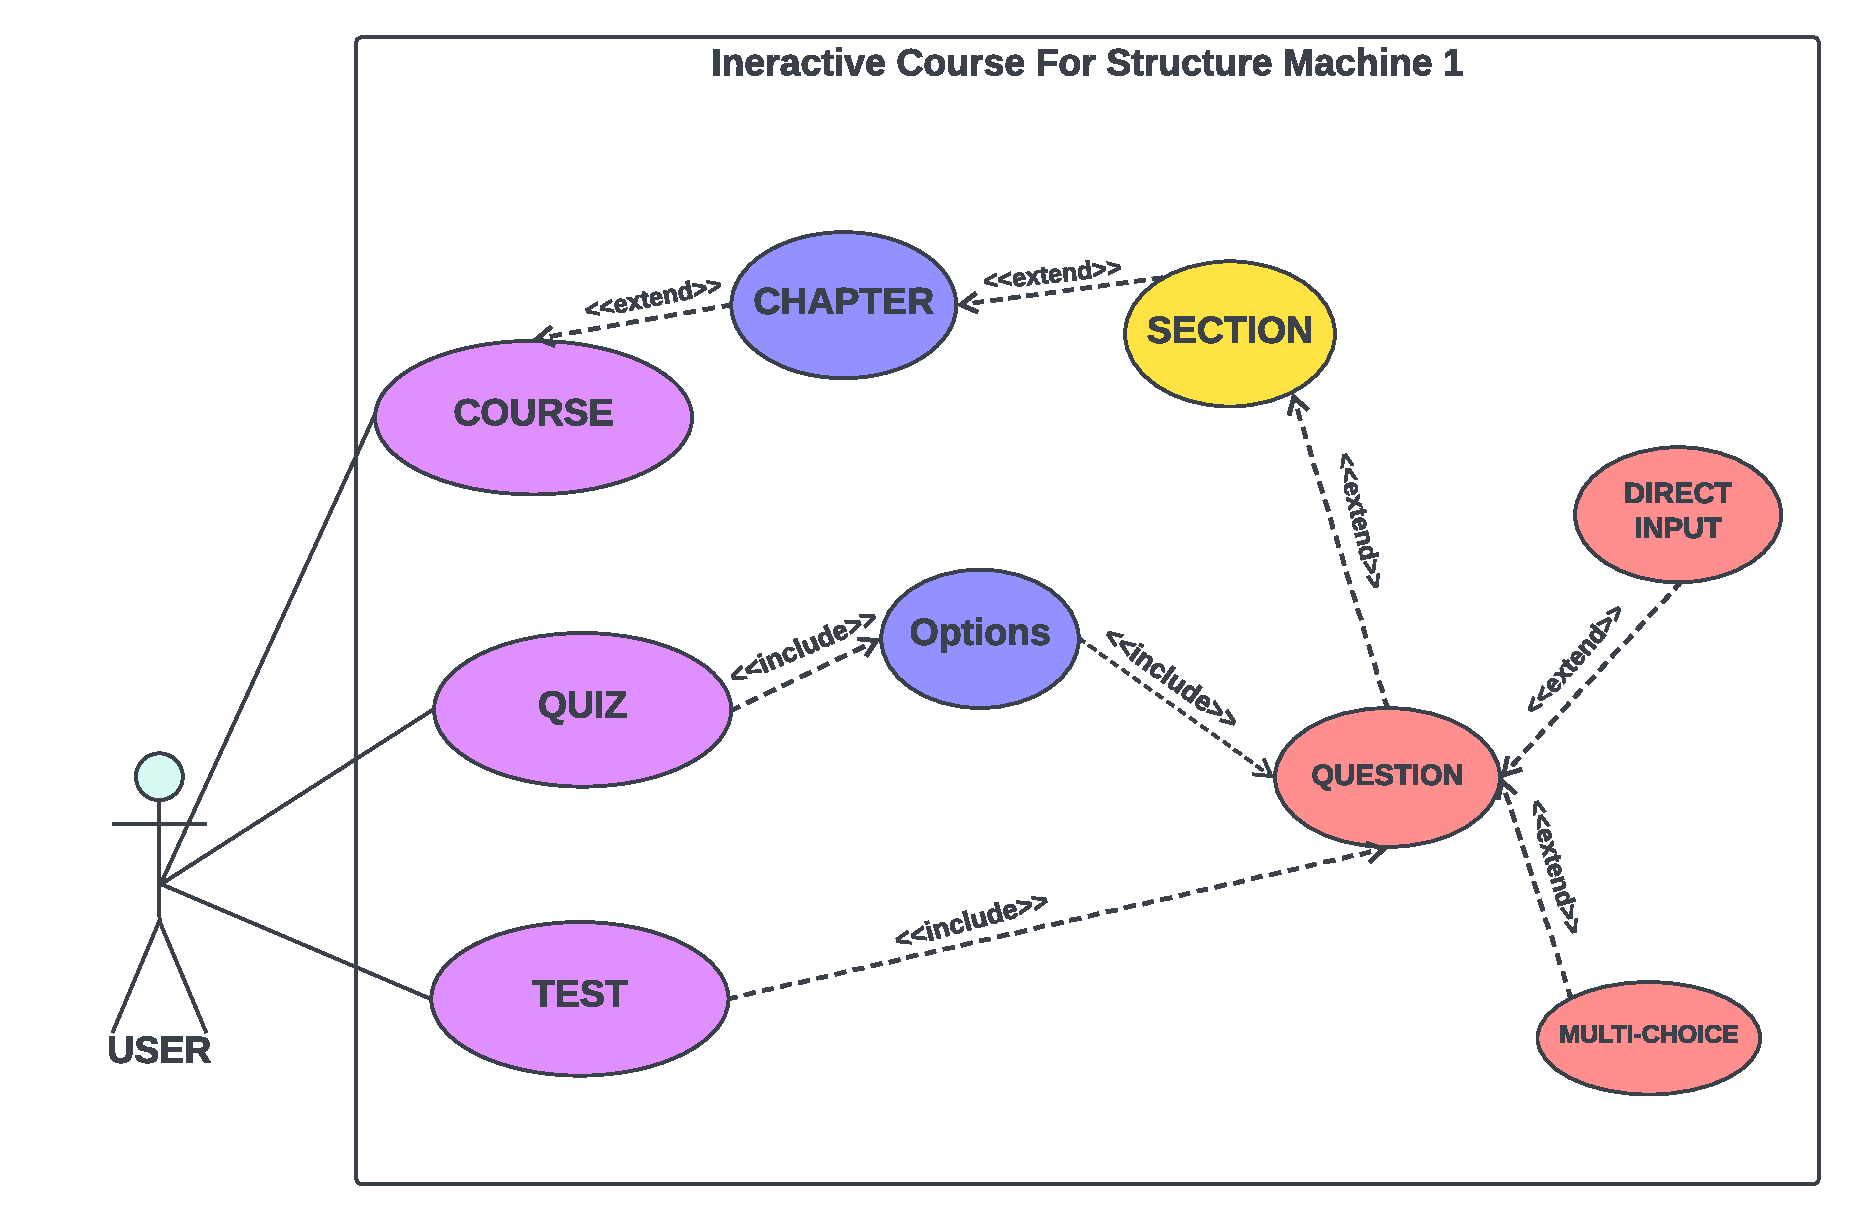
\includegraphics[scale=0.5]{img/Use Case.pdf}                
	\caption{Use Case diagram.} 
	\label{fig:UseCaseD}
\end{figure*} 
%===================================================================

\subsection{Sequence diagrams:}
A sequence diagram, in the context of UML, represents object collaboration and is used to define event sequences between objects for a certain outcome, it is an essential component used in processes related to analysis, design and documentation.\cite{Techopedia-DS} \\\\
A sequence diagram is also known as a timing diagram, event diagram and event scenario.\cite{Techopedia-DS}

\subsection{COURSE:}
This first scenario shows how user can see the hole CHAPTERS of the course, and try  a question with a specific type depends on the chapter's TITLE.

\newpage

\begin{table}[h!]
	\begin{center}
		\begin{tabular}{ |p{3cm}|p{9cm}|  }
 		\hline
 		\multicolumn{2}{|c|}{Identication summary} \\
 		\hline
 		Use Case Title & COURSE. \\
 		\hline
 		Abstract   & User learn course. \\
		\hline
 		Actor&  User. \\
		\hline
		\multicolumn{2}{|c|}{Identication summary} \\
		\hline
		Preconditions & Accessible system.  \\
		\hline
		User exists    &  The purpose of this system is navigate and learn from the course. \\
		\hline
		Scenario &  1- User clicks on Course button. \\ & 2- System loads all chapters. \\ & 3- System shows the names of chapters. \\ & 4- User chooses chapter. \\ & 5- System loads titles of chapter . \\ & 6- System shows the content of titles . \\ & 7- User clicks on Try. \\ & 8- System sends SQL requeste (Select title's question) to DataBase.\\ & 9- Database return data(title's question).\\ & 10- System loads results.\\ & 11- System shows results.\\
		\hline
		Object& User learn the course with live examples.   \\
 		\hline
\end{tabular}
\end{center}
\caption{Text Description of Use Case "COURSE".}
\label{tab:DS COURSE}
\end{table}



\newpage
The figure \ref{fig:COURSE DS} represents COURSE Sequence diagram.
%***************************************************
\begin{figure*}[ht]
	\centering
	\label{}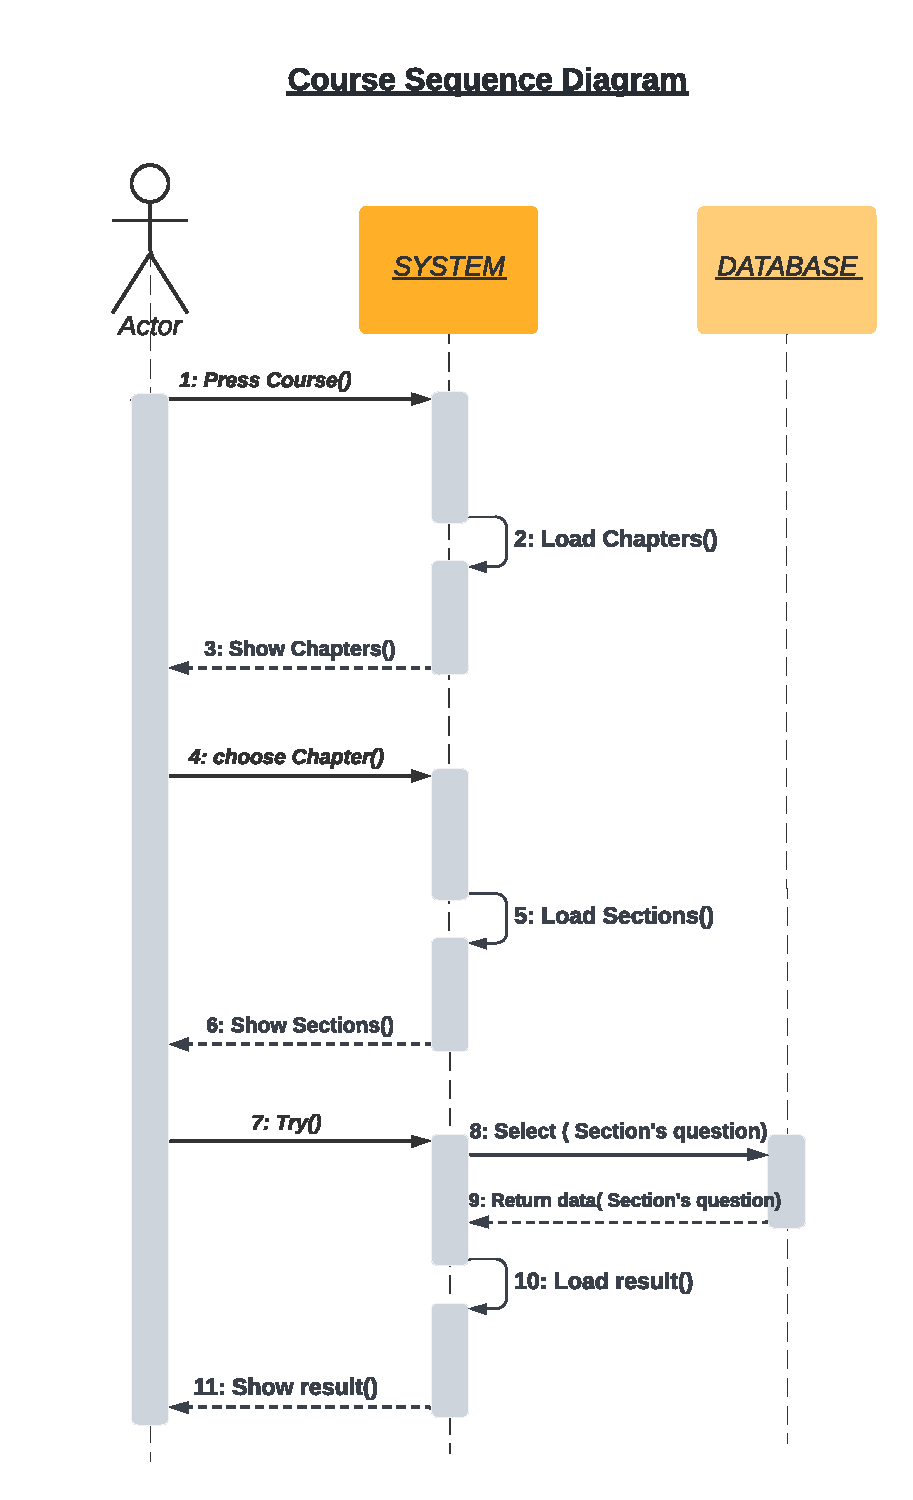
\includegraphics[scale=0.6]{img/Course Sequence diagram.pdf}                
	\caption{COURSE Sequence diagram.} 
	\label{fig:COURSE DS}
\end{figure*} 
%===================================================================






\subsection{QUIZ:}
This second scenario shows how user can test what he learned in this course with a specific Options (choose chapters and number of questions).
\newpage

\begin{table}[h!]
	\begin{center}
		\begin{tabular}{ |p{3cm}|p{9cm}|  }
			\hline
			\multicolumn{2}{|c|}{Identication summary} \\
			\hline
			Use Case Title & QUIZ. \\
			\hline
			Abstract   & User takes a quiz. \\
		   \hline
			Actor&  User. \\
		   \hline
		   \multicolumn{2}{|c|}{Identication summary} \\
		   \hline
		   Preconditions & Accessible system.  \\
		   \hline
		   User exists    &  The purpose of this system is taking a quiz. \\
		   \hline
		   Scenario &  1- User clicks on Quiz button. \\ & 2- System loads Options. \\ & 3- System shows Options. \\ & 4- User chooses options. \\ & 5- System shows Start button . \\ & 6- User clicks on Start button . \\ & 7- System sends SQL requeste (Select Questions) to DataBase . \\ & 8- Database return data(Questions) .\\ & 9- System loads Quiz results.\\ & 10- System shows Quiz results.\\
		   \hline
		   Object&  User can take a quiz with any options he wants .  \\
			\hline
\end{tabular}
\end{center}
\caption{Text Description of Use Case "QUIZ".}
\label{tab:DS QUIZ}
\end{table}



\newpage
The figure \ref{fig:QUIZ DS} represents QUIZ Sequence diagram.
%***************************************************
\begin{figure*}[ht]
	\centering
	\label{}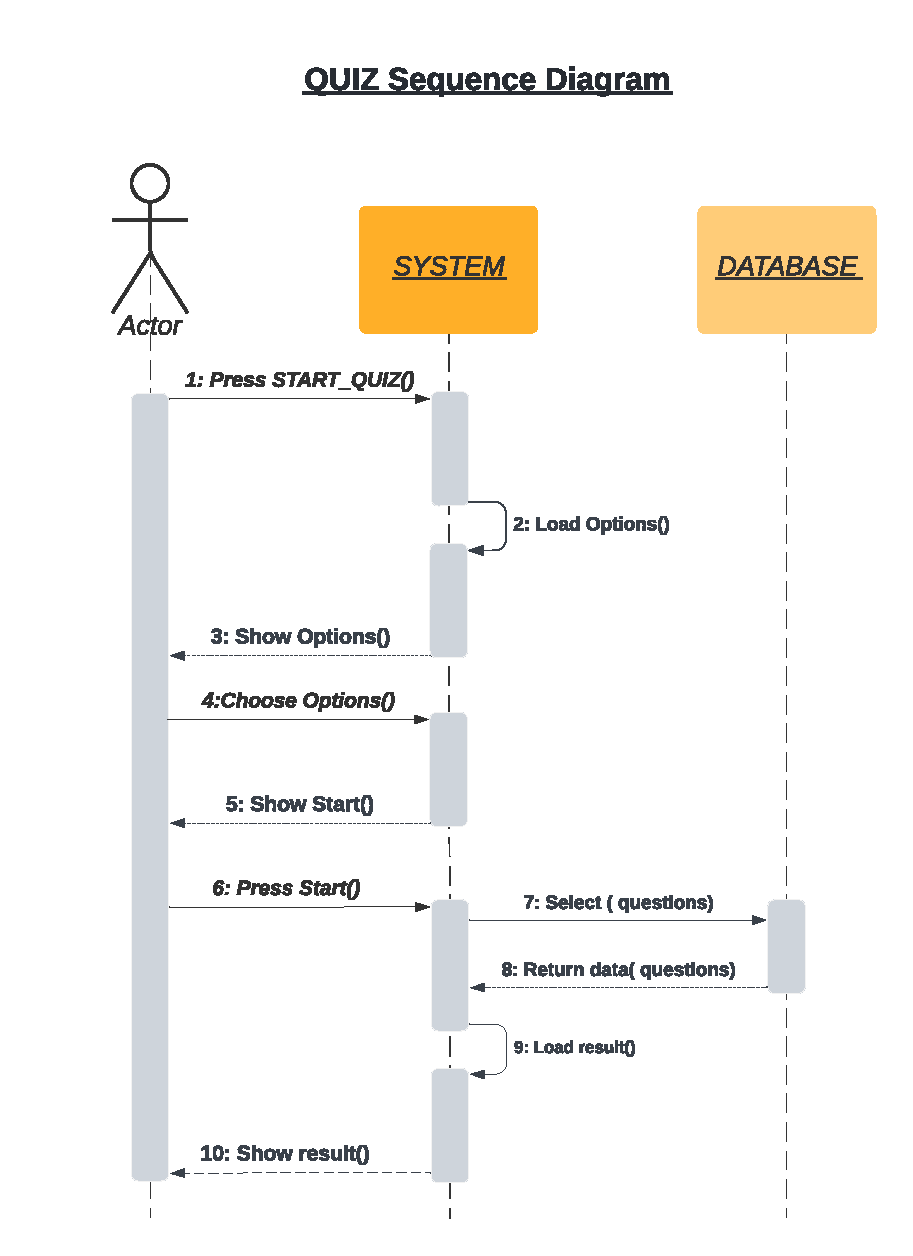
\includegraphics[scale=0.7]{img/Quiz Sequence diagram.pdf}                
	\caption{QUIZ Sequence diagram.} 
	\label{fig:QUIZ DS}
\end{figure*} 
%===================================================================







\subsection{TEST:}
This third scenario shows how user can find a practical models for machine structure tests including the hole course .
\newpage

\begin{table}[h!]
	\begin{center}
		\begin{tabular}{ |p{3cm}|p{9cm}|  }
			\hline
			\multicolumn{2}{|c|}{Identication summary} \\
			\hline
			Use Case Title & Test. \\
			\hline
			Abstract   & User takes a Test. \\
		   \hline
			Actor&  User. \\
		   \hline
		   \multicolumn{2}{|c|}{Identication summary} \\
		   \hline
		   Preconditions & Accessible system.  \\
		   \hline
		   User exists    &  The purpose of this system is taking a Test. \\
		   \hline
		   Scenario &  1- User clicks on Test button. \\ & 2- System shows Start button . \\ & 3- User clicks on Start button . \\ & 4- System sends SQL requeste (Select Question from each chapter) to DataBase . \\ & 5- Database return data(Question from each chapter) .\\ & 6- System loads Test results.\\ & 7- System shows Test results.\\
		   \hline
		   Object&  user can find a practical models for machine structure tests including the hole course. \\
			\hline
\end{tabular}
\end{center}
\caption{Text Description of Use Case "TEST".}
\label{tab:DS TEST}
\end{table}



\newpage
The figure \ref{fig:TEST DS} represents TEST Sequence diagram.
%***************************************************
\begin{figure*}[ht]
	\centering
	\label{}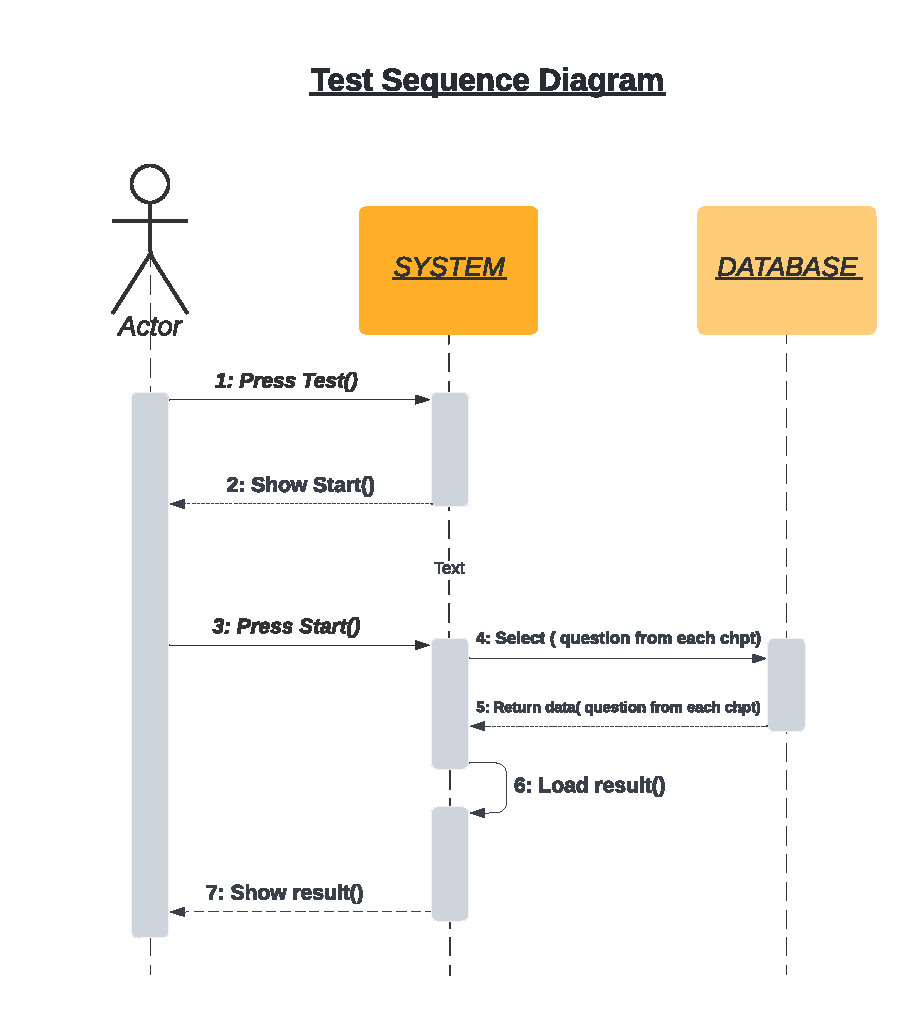
\includegraphics[scale=0.7]{img/Test Sequence diagram.pdf}                
	\caption{TEST Sequence diagram.} 
	\label{fig:TEST DS}
\end{figure*} 
%===================================================================



\subsection{ABOUT:}
This last scenario shows how user can find more details and informations of this system's developers .
\newpage

\begin{table}[h!]
	\begin{center}
		\begin{tabular}{ |p{3cm}|p{9cm}|  }
			\hline
			\multicolumn{2}{|c|}{Identication summary} \\
			\hline
			Use Case Title & About. \\
			\hline
			Abstract   & User sees about. \\
		   \hline
			Actor&  User. \\
		   \hline
		   \multicolumn{2}{|c|}{Identication summary} \\
		   \hline
		   Preconditions & Accessible system.  \\
		   \hline
		   User exists    &  The purpose of this system is see who developedthis system. \\
		   \hline
		   Scenario &  1- User clicks on About button. \\ & 2- System loads content . \\ & 3- System shows content . \\ 
		   \hline
		   Object&  user can find more details and informations of this system's developers .\\
			\hline
\end{tabular}
\end{center}
\caption{Text Description of Use Case "ABOUT".}
\label{tab:DS ABOUT}
\end{table}



\newpage
The figure \ref{fig:ABOUT DS} represents TEST Sequence diagram.
%***************************************************
\begin{figure*}[ht]
	\centering
	\label{}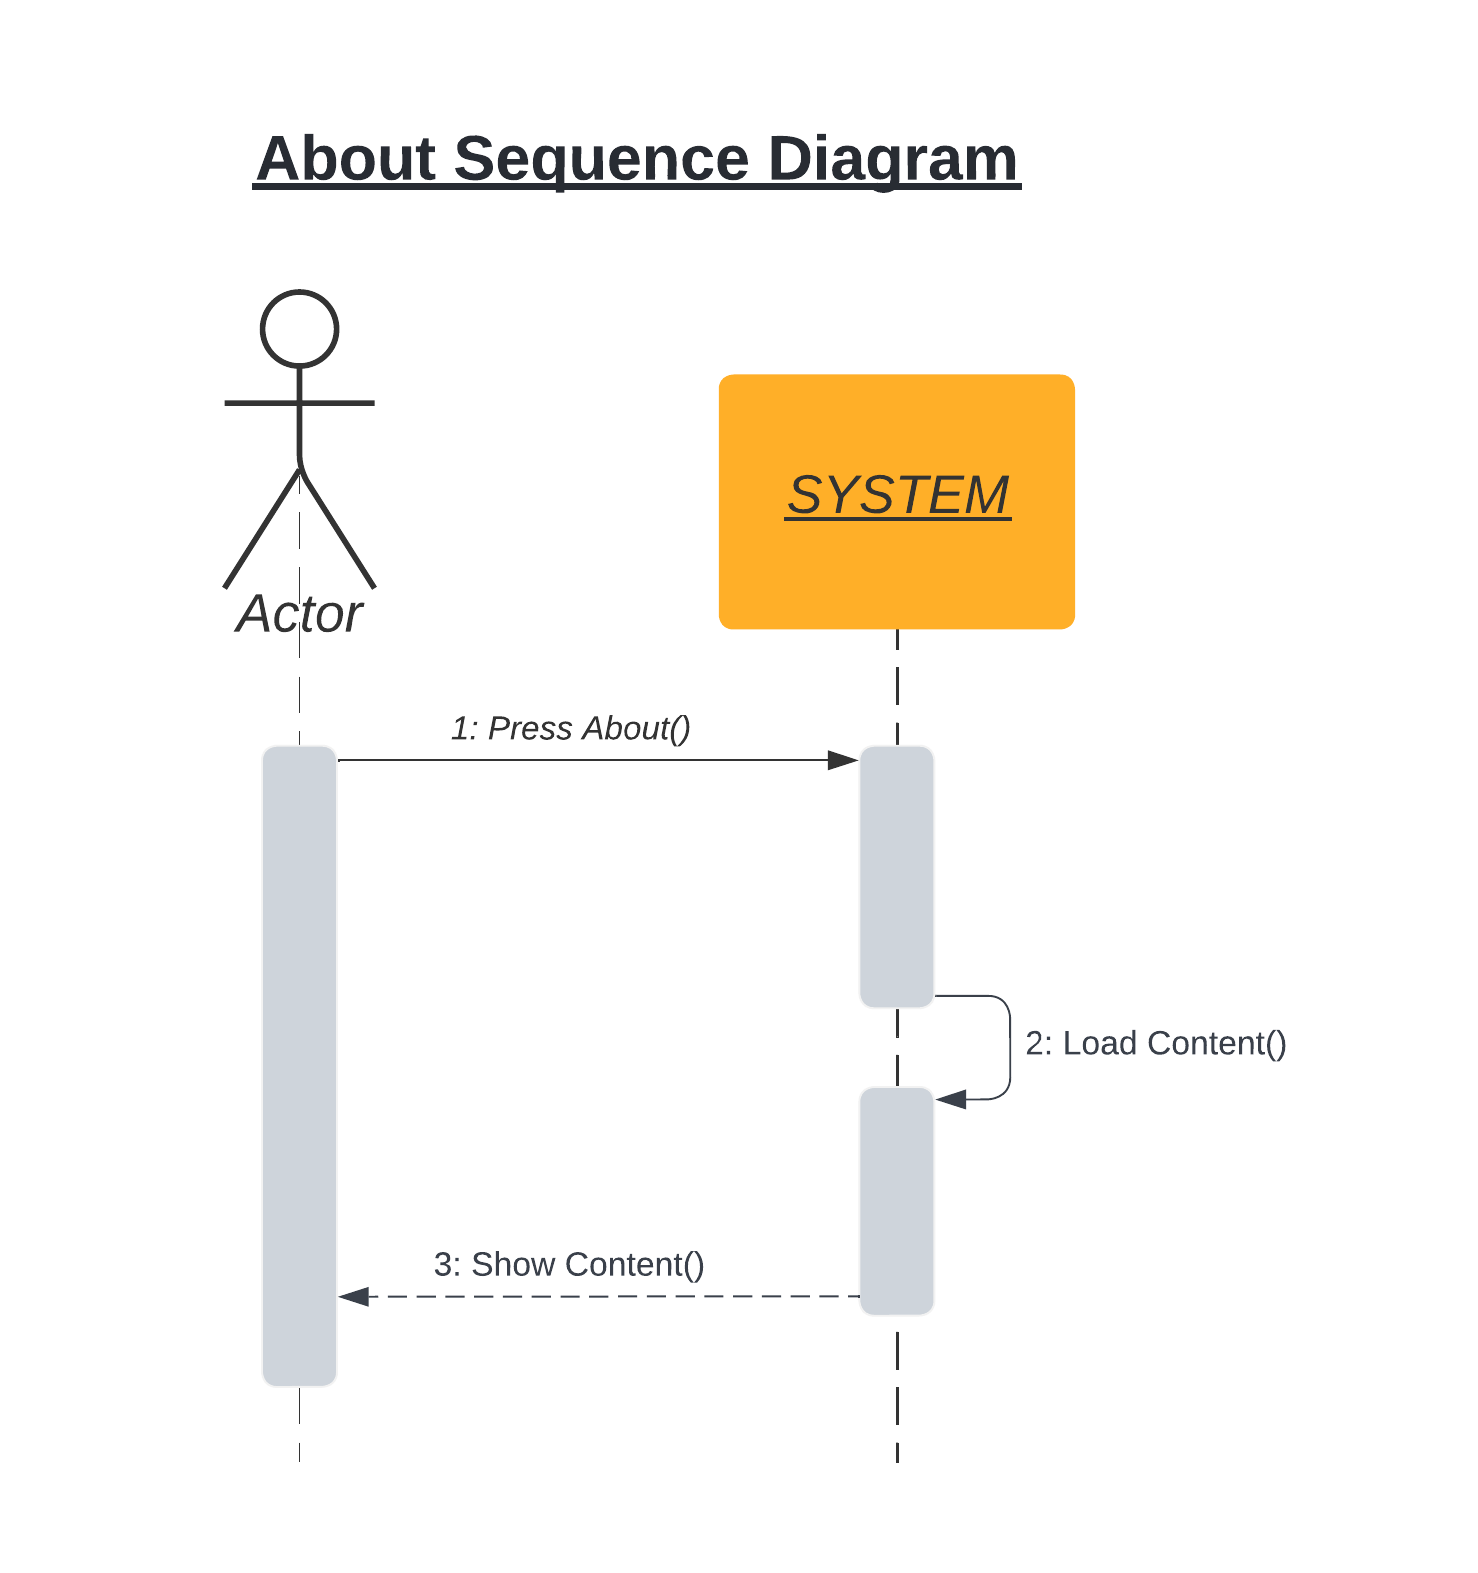
\includegraphics[scale=0.2]{img/About Sequence diagram.png}                
	\caption{ABOUT Sequence diagram.} 
	\label{fig:ABOUT DS}
\end{figure*} 
%===================================================================


\subsection{Class Diagram:}
A class diagram is a type of diagram and part of a unified modeling language (UML) that defines and provides the overview and structure of a system in terms of classes, attributes and methods, and the relationships between different classes. \\
It is used to illustrate and create a functional diagram of the system classes and serves as a system development resource within the software development life cycle. \cite{Techopedia-DC} \\
\newpage

\subsubsection{Why Class Diagram?}
A class diagram is primarily designed for developers to provide the conceptual model and architecture of the system being developed. Typically, a class diagram consists of more than one class or all the created classes for a system. \cite{Techopedia-DC} \\
It is a type of structure diagram and looks similar to a flow chart having three main parts illustrated in rectangular boxes. The first or top part specifies the class name, the second or middle specifies attributes of that class and the third or bottom section lists the methods or operations that specific class can perform. \cite{Techopedia-DC} \\

The figure \ref{fig:DC} represents this system's Class Diagram.


%***************************************************
\begin{figure*}[ht]
	\centering
	\label{}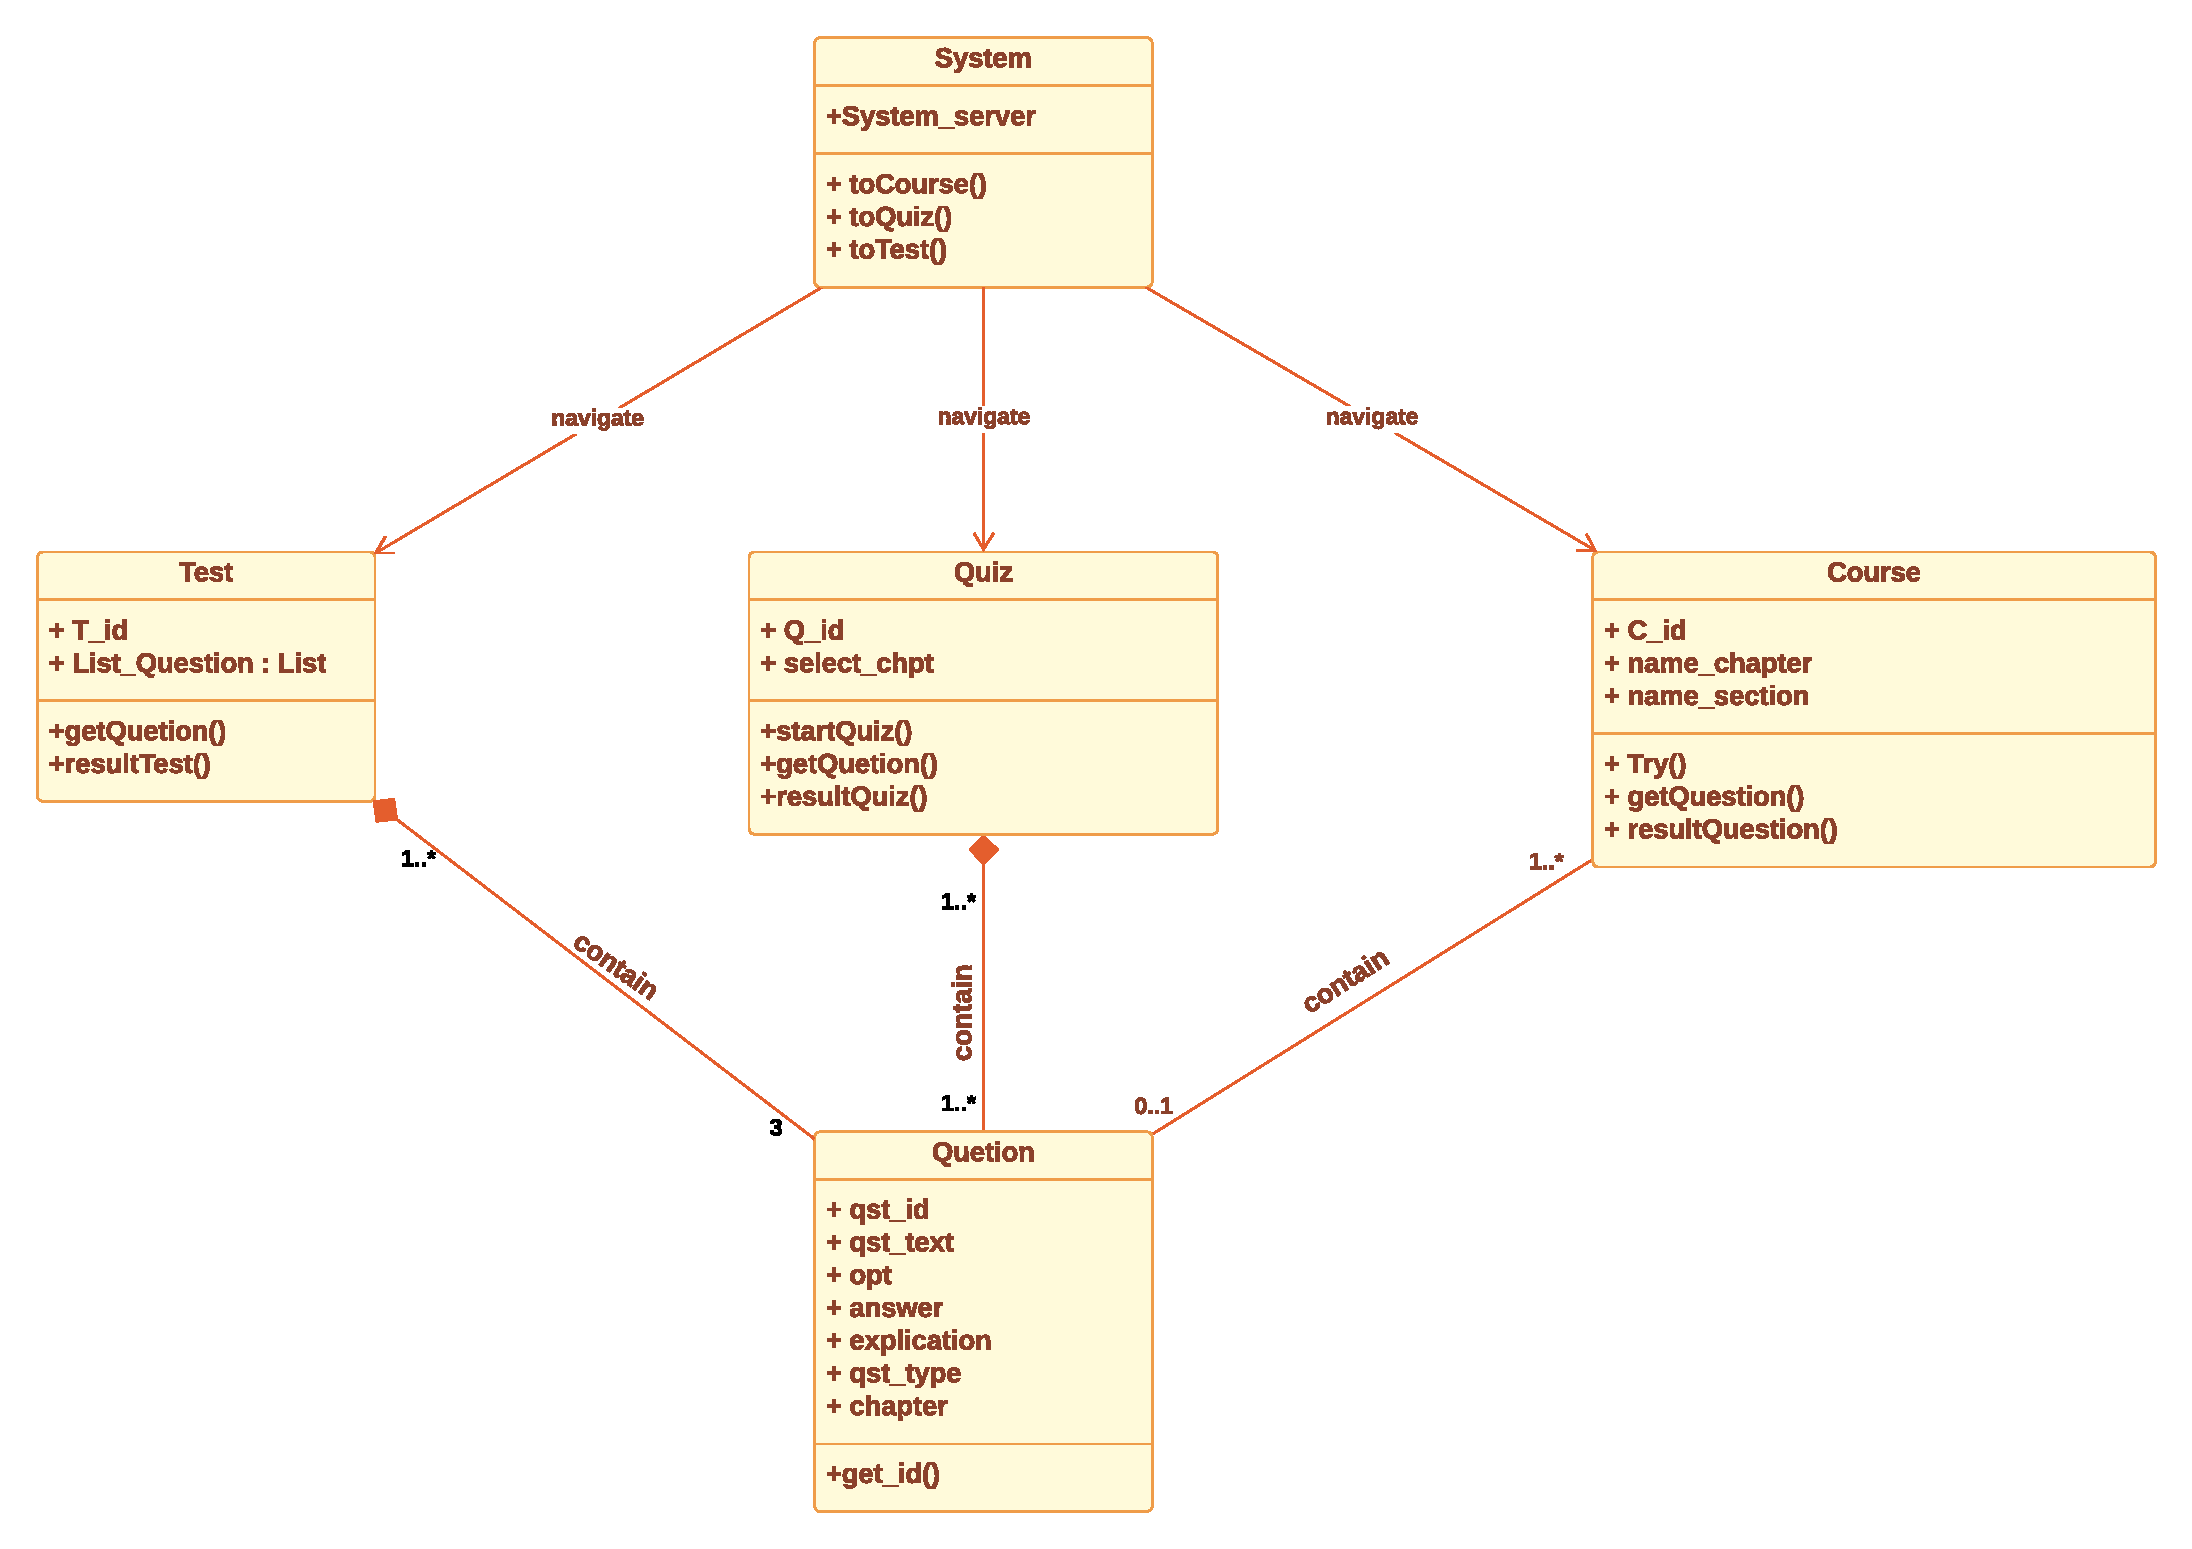
\includegraphics[scale=0.45]{img/UML class.pdf}                
	\caption{Class Diagram.} 
	\label{fig:DC}
\end{figure*} 
%===================================================================



\newpage
The table \ref{tab:DC} represents classes and attributes as well as their types and description .

\begin{table}[h!]
	\begin{center}
		\begin{tabular}{ |p{3cm}|p{3cm}|p{4cm}|p{2cm}|  }
 		\hline
 		Class & attributes & Description & Type \\
 		\hline \hline
 		System & System-server & system's identificator & Digital \\
 		\hline
 		Course & C-id & Course identificator & Digital  \\
			& name-chapter & chapter's name & Alphabetic \\
			& name-title & title's name & Alphabetic \\
		\hline
		Quiz & Q-id & Quiz identificator & Digital  \\
			& select-chpt & choosing chapter & Digital \\
			& nbr-qst & number of questions & Digital \\
		\hline
		Test & T-id & Test identificator & Digital  \\
			& List-Question & List of questions & Alphabetic \\
			& all-chpt & choosing from all chapters & Digital \\
		\hline
		Question & qst-id & Question identificator & Digital  \\
			& nbr-qst & number of questions & Digital \\
			& select-chpt & choosing chapter & Digital \\
			& name-chapter & chapter's name & Alphabetic \\
			& name-title & title's name & Alphabetic \\
			& all-chpt & choosing from all chapters & Digital \\
		\hline
\end{tabular}
\end{center}
\caption{Description of Class Diagram.}
\label{tab:DC}
\end{table}


\newpage

\subsubsection{Database's Class Diagram:}

The figure \ref{fig:BDD DC} represents the database in the form of a class diagram.\\\\\\

%***************************************************
\begin{figure*}[ht]
	\centering
	\label{}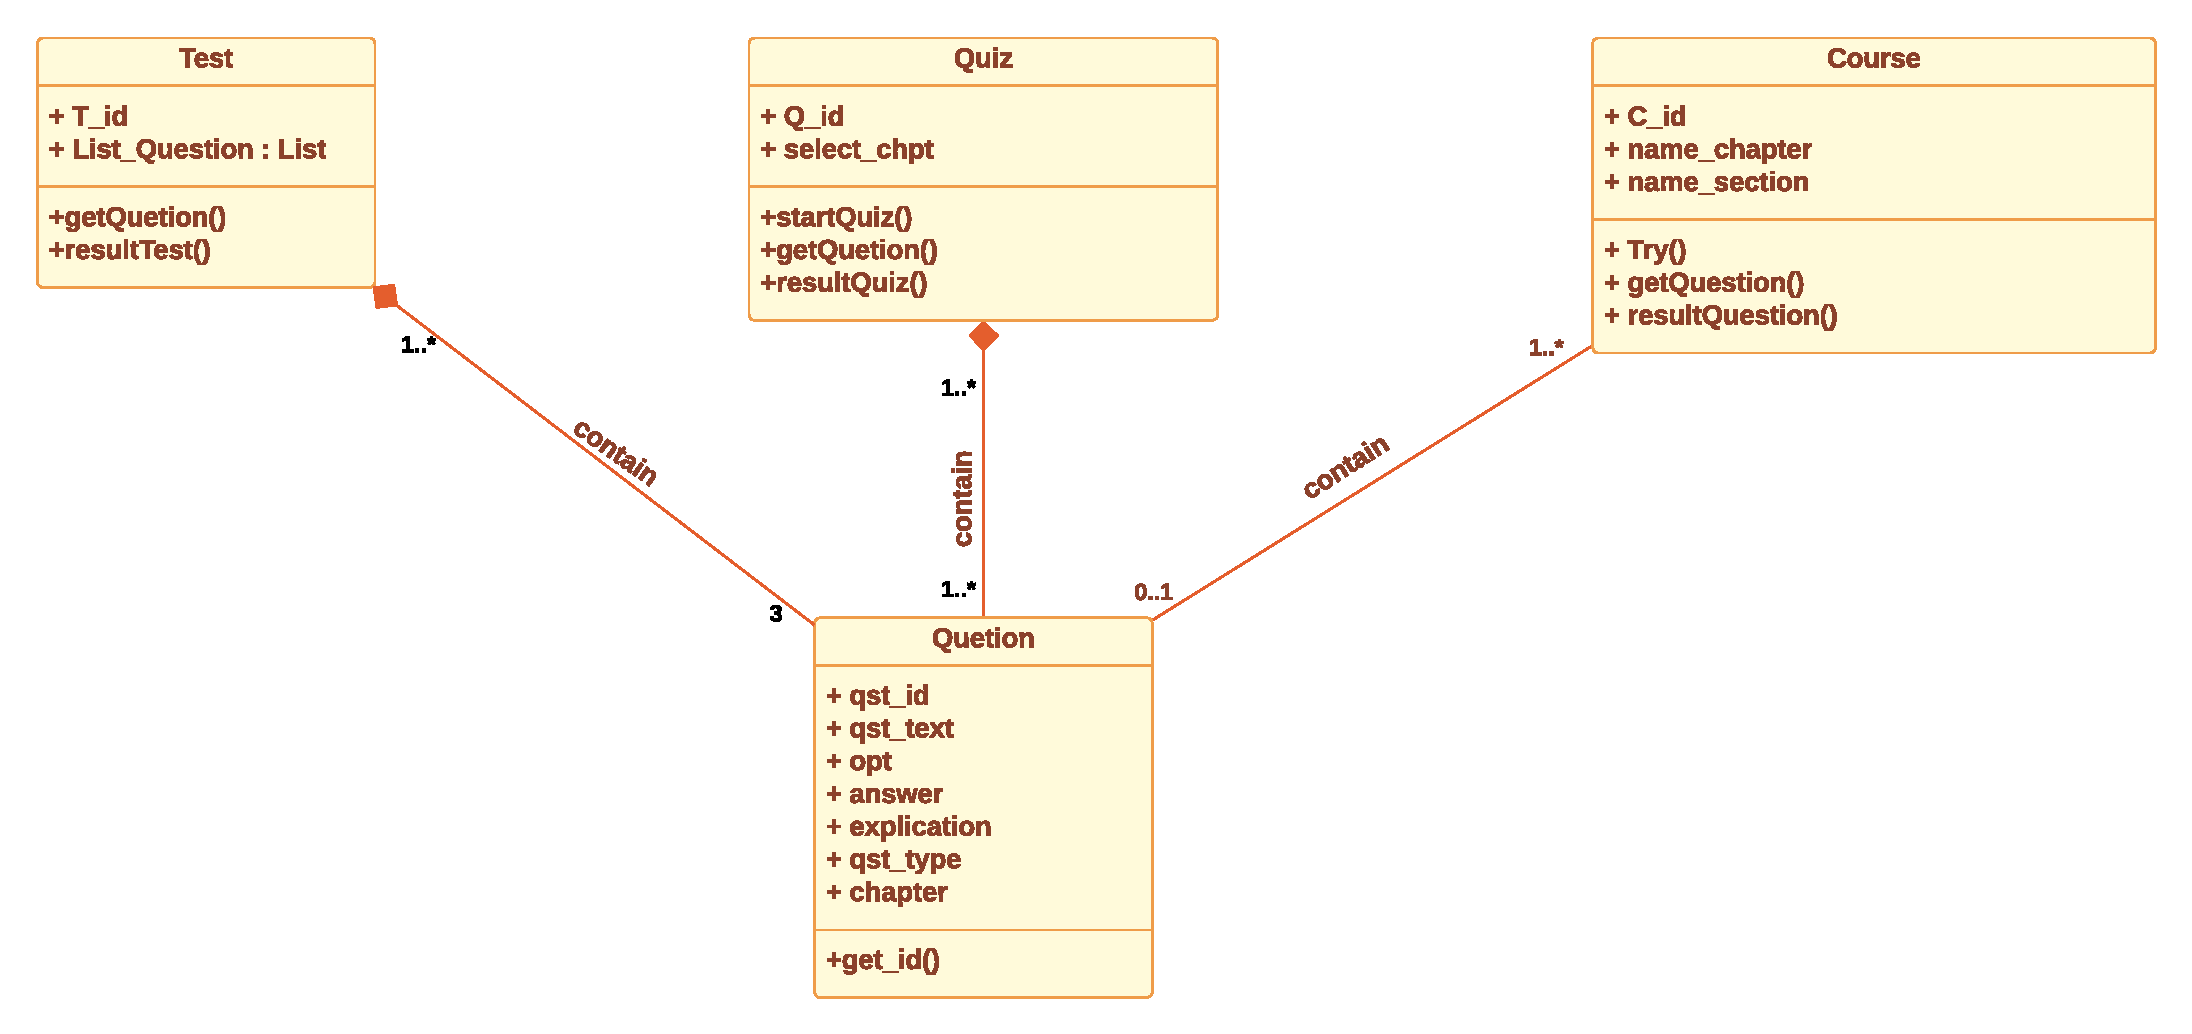
\includegraphics[scale=0.45]{img/BDD class.pdf}                
	\caption{Database's Class Diagram.} 
	\label{fig:BDD DC}
\end{figure*} 
%===================================================================



The table \ref{tab:BDD DC} represents classes and attributes of database's class diagram as well as their types and description .\\\\\\
\newpage
\begin{table}[h!]
	\begin{center}
		\begin{tabular}{ |p{3cm}|p{3cm}|p{4cm}|p{2cm}|  }
 		\hline
 		Class & attributes & Description & Type \\
 		\hline \hline
 		Course & C-id & Course identificator & Digital  \\
			& name-chapter & chapter's name & Alphabetic \\
			& name-title & title's name & Alphabetic \\
		\hline
		Quiz & Q-id & Quiz identificator & Digital  \\
			& select-chpt & choosing chapter & Digital \\
			& nbr-qst & number of questions & Digital \\
		\hline
		Test & T-id & Test identificator & Digital  \\
			& List-Question & List of questions & Alphabetic \\
			& all-chpt & choosing from all chapters & Digital \\
		\hline
		Question & qst-id & Question identificator & Digital  \\
			& nbr-qst & number of questions & Digital \\
			& select-chpt & choosing chapter & Digital \\
			& name-chapter & chapter's name & Alphabetic \\
			& name-title & title's name & Alphabetic \\
			& all-chpt & choosing from all chapters & Digital \\
		\hline
\end{tabular}
\end{center}
\caption{Description of Database's Class Diagram.}
\label{tab:BDD DC}
\end{table}


\subsection{The relational model and creation of the Database:}

A relational data model involves the use of data tables that collect groups of elements into relations. These models work based on the idea that each table setup will include a primary key or identifier. Other tables use that identifier to provide "relational" data links and results. Database administrators use something called Structured Query Language (SQL) to retrieve data elements from a relational database.\cite{Techopedia-relational-model} \\
Course(C-id,//name-chapter,//name-title).\\
Quiz(Q-id,//select-chpt,//nbr-qst).\\
Test(T-id,List-Question,//all-chpt).\\
Question(qst-id,nbr-qst,select-chpt,name-chapter,name-title,all-chpt).\\


\section{Conclusion:}
This chapter defined the basic steps for developing the system where specified functional and
non-functional requirements using the concepts of Unified Modeling Language ( Use Case
diagram, Sequence diagrams, and Class diagram), and clarified the goal of the analysis and
design. Next step is realizing the system
by introducing the programming languages, tools, and development environment used on
implementation.\\








\chapter{Implementation and evaluation}
\lhead{\textit{Chapitre \thechapter}}
\rhead{\textit{Implementation and evaluation}}

\section{ Introduction:}
Lorem ipsum dolor sit amet, consectetur adipisicing elit, sed do eiusmod
tempor incididunt ut labore et dolore magna aliqua. Ut enim ad minim veniam,
quis nostrud exercitation ullamco laboris nisi ut aliquip ex ea commodo
consequat. Duis aute irure dolor in reprehenderit in voluptate velit esse
cillum dolore eu fugiat nulla pariatur. Excepteur sint occaecat cupidatat non
proident, sunt in culpa qui officia deserunt mollit anim id est laborum.


\section{Work environment:}
Lorem ipsum dolor sit amet, consectetur adipisicing elit, sed do eiusmod
tempor incididunt ut labore et dolore magna aliqua. Ut enim ad minim veniam,
quis nostrud exercitation ullamco laboris nisi ut aliquip ex ea commodo
consequat. Duis aute irure dolor in reprehenderit in voluptate velit esse
cillum dolore eu fugiat nulla pariatur. Excepteur sint occaecat cupidatat non
proident, sunt in culpa qui officia deserunt mollit anim id est laborum.

\subsection{Hardware:}
For programming we used a laptop, as for testing we used mobile phones, laptops, tabeltes and even a smart tv to monitor the performance of the website on them. The characteristics of
these devices are:
\begin{itemize}
	\item LENOVO laptop(for programming):
	\begin{itemize}
		\item Processor : Intel (R) Core (TM) i7-7600U CPU @ 2.80 GHz(4 CPUs), ~2.90 GHz.
		\item RAM : 16 GB.
		\item System : Windows 10 Pro - 64 Bit.
	\end{itemize}
	\item Consectetur adipisicing elit;
	\item Fin.
\end{itemize}


\subsection{Software:}
\indent \textbf{Visual Studio Code:\\}
 Visual Studio Code is not just another evolved Notepad with syntax colorization and automatic indentation. Instead, it is a very powerful code-focused development
 environment expressly designed to make it easier to write web, mobile, and cloud applications using languages that are available to different development platforms and
  to support the application development life cycle with a built-in debugger and integrated support for the popular Git version control engine.\cite{Del_Sole2021-cv}\\

\textbf{Sublime Text:\\}
 Sublime Text is a proprietary, cross-platform text editor designed for people who spend huge amounts of time shuffling code around. A programmer's editor,
 Sublime Text is a third option to the long-standing “Vi or Emacs” conundrum. Going beyond the basics of syntax highlighting and code folding, Sublime offers a 
 litany of innovative and unique features. With version 3.0 just around the corner, I'm taking you on a tour of Sublime's most compelling features and add-on packages.\cite{kinder2013sublime}\\


 \textbf{XAMPP:\\}
 \indent XAMPP is a small and light Apache distribution containing the most common web development
 technologies in a single package. Its contents, small size, and portability make it the ideal tool for
 students developing and testing applications in PHP and MySQL. XAMPP is available as a free
 download in two specific packages: full and lite. While the full package download provides a wide
 array of development tools, this article will focus on using XAMPP Lite which contains the necessary
 technologies that meet the Ontario Skills Competition standards. As the name implies, the light version
 is a small package containing Apache HTTP Server, PHP, MySQL, phpMyAdmin, Openssl, and
 SQLite.\cite{dvorski2007installing}\\



Bla bla bla bla bla (voir Figure~\ref{fig:Results})
%+++++++++++++++++++++++++++++++++++++++++++++++++++++
 \begin{figure*} [ht]
 	\centering
 	\subfloat[user$_1$]{\label{}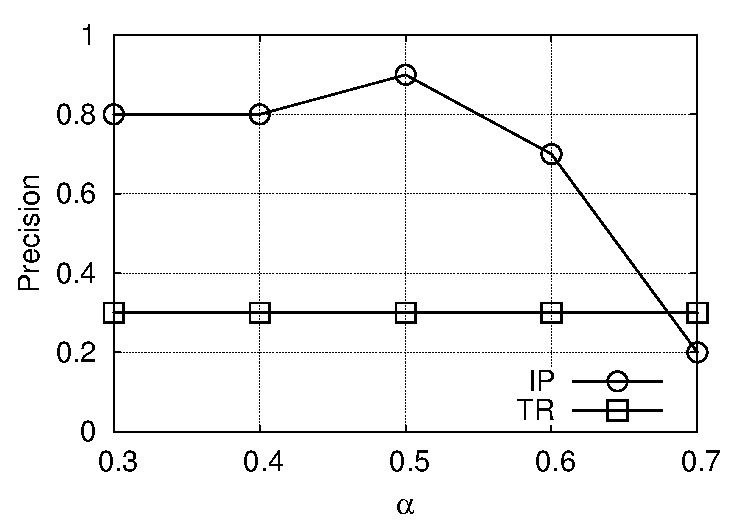
\includegraphics[scale=0.5]{img/pVSa1-eps-converted-to.pdf}}                
 	\subfloat[user$_2$]{\label{}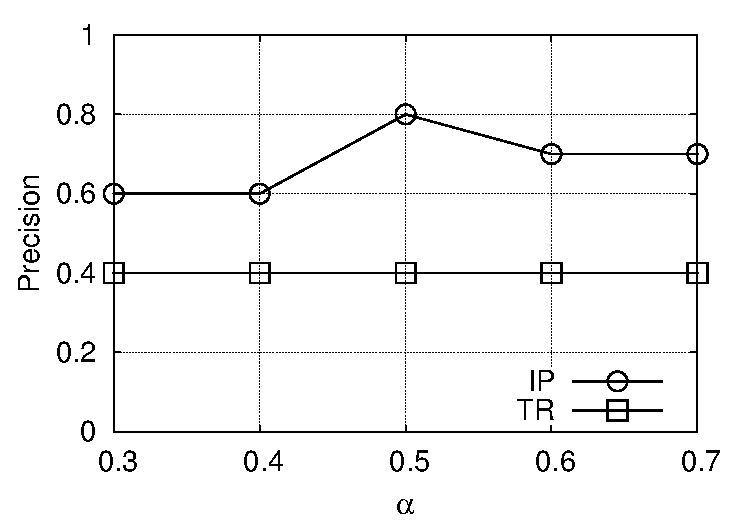
\includegraphics[scale=0.5]{img/pVSa2-eps-converted-to.pdf}}\\
 	\subfloat[user$_3$]{\label{}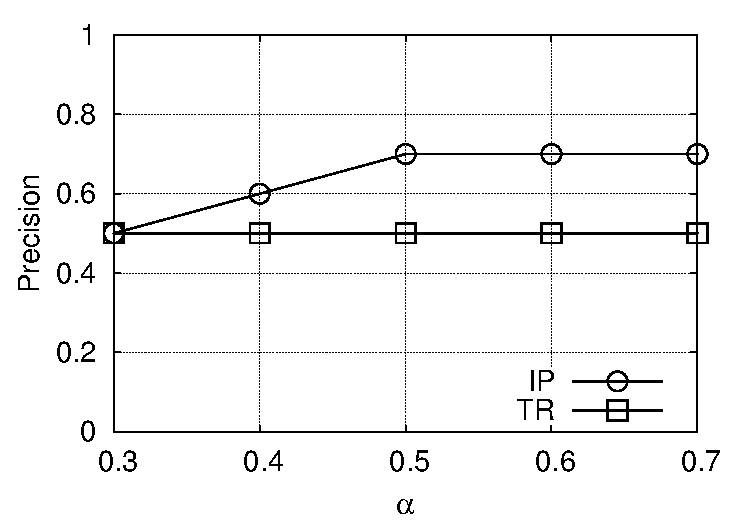
\includegraphics[scale=0.5]{img/pVSa3-eps-converted-to.pdf}}
 	\subfloat[user$_4$]{\label{}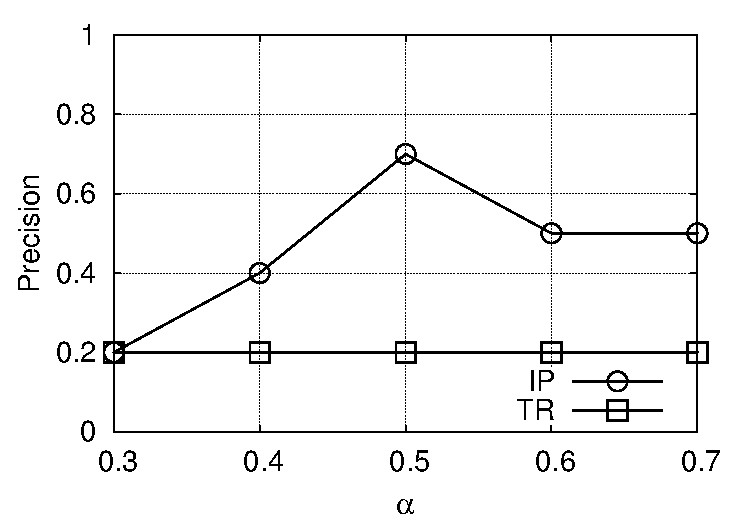
\includegraphics[scale=0.5]{img/pVSa4-eps-converted-to.pdf}}
 	\caption{Precision vs $\alpha$} 
 	\label{Results}
 \end{figure*}
 %
 %++++++++++++++++++++++++++++++++++++++++++++++++++++
\subsection{Une sous section}
Lorem ipsum dolor sit amet, consectetur adipisicing elit, sed do eiusmod
tempor incididunt ut labore et dolore magna aliqua. Ut enim ad minim veniam,
quis nostrud exercitation ullamco laboris nisi ut aliquip ex ea commodo
consequat. Duis aute irure dolor in reprehenderit in voluptate velit esse
cillum dolore eu fugiat nulla pariatur. Excepteur sint occaecat cupidatat non
proident, sunt in culpa qui officia deserunt mollit anim id est laborum.

\subsection{Une une autre sous section}
Lorem ipsum dolor sit amet, consectetur adipisicing elit, sed do eiusmod
tempor incididunt ut labore et dolore magna aliqua. Ut enim ad minim veniam,
quis nostrud exercitation ullamco laboris nisi ut aliquip ex ea commodo
consequat. Duis aute irure dolor in reprehenderit in voluptate velit esse
cillum dolore eu fugiat nulla pariatur. Excepteur sint occaecat cupidatat non
proident, sunt in culpa qui officia deserunt mollit anim id est laborum.

\begin{itemize}
	\item Lorem ipsum dolor sit amet;
	\item Consectetur adipisicing elit;
	\item Fin.
\end{itemize}

\subsubsection{Une sous sous section}
Lorem ipsum dolor sit amet, consectetur adipisicing elit, sed do eiusmod
tempor incididunt ut labore et dolore magna aliqua. Ut enim ad minim veniam,
quis nostrud exercitation ullamco laboris nisi ut aliquip ex ea commodo
consequat. Duis aute irure dolor in reprehenderit in voluptate velit esse
cillum dolore eu fugiat nulla pariatur. Excepteur sint occaecat cupidatat non
proident, sunt in culpa qui officia deserunt mollit anim id est laborum.

\paragraph{Un paragraphe}
Lorem ipsum dolor sit amet, consectetur adipisicing elit, sed do eiusmod
tempor incididunt ut labore et dolore magna aliqua. Ut enim ad minim veniam,
quis nostrud exercitation ullamco laboris nisi ut aliquip ex ea commodo
consequat. Duis aute irure dolor in reprehenderit in voluptate velit esse
cillum dolore eu fugiat nulla pariatur. Excepteur sint occaecat cupidatat non
proident, sunt in culpa qui officia deserunt mollit anim id est laborum.

\section{Une deuxième section principale}
Lorem ipsum dolor sit amet, consectetur adipisicing elit, sed do eiusmod
tempor incididunt ut labore et dolore magna aliqua. Ut enim ad minim veniam,
quis nostrud exercitation ullamco laboris nisi ut aliquip ex ea commodo
consequat. Duis aute irure dolor in reprehenderit in voluptate velit esse
cillum dolore eu fugiat nulla pariatur. Excepteur sint occaecat cupidatat non
proident, sunt in culpa qui officia deserunt mollit anim id est laborum.

\subsection{Une sous section}
Lorem ipsum dolor sit amet, consectetur adipisicing elit, sed do eiusmod
tempor incididunt ut labore et dolore magna aliqua. Ut enim ad minim veniam,
quis nostrud exercitation ullamco laboris nisi ut aliquip ex ea commodo
consequat. Duis aute irure dolor in reprehenderit in voluptate velit esse
cillum dolore eu fugiat nulla pariatur. Excepteur sint occaecat cupidatat non
proident, sunt in culpa qui officia deserunt mollit anim id est laborum.

\subsection{Une autre sous section}
Lorem ipsum dolor sit amet, consectetur adipisicing elit, sed do eiusmod
tempor incididunt ut labore et dolore magna aliqua. Ut enim ad minim veniam,
quis nostrud exercitation ullamco laboris nisi ut aliquip ex ea commodo
consequat. Duis aute irure dolor in reprehenderit in voluptate velit esse
cillum dolore eu fugiat nulla pariatur. Excepteur sint occaecat cupidatat non
proident, sunt in culpa qui officia deserunt mollit anim id est laborum.

\subsection{Une autre sous section}
Lorem ipsum dolor sit amet, consectetur adipisicing elit, sed do eiusmod
tempor incididunt ut labore et dolore magna aliqua. Ut enim ad minim veniam,
quis nostrud exercitation ullamco laboris nisi ut aliquip ex ea commodo
consequat. Duis aute irure dolor in reprehenderit in voluptate velit esse
cillum dolore eu fugiat nulla pariatur. Excepteur sint occaecat cupidatat non
proident, sunt in culpa qui officia deserunt mollit anim id est laborum.

\section{Conclusion}
Lorem ipsum dolor sit amet, consectetur adipisicing elit, sed do eiusmod
tempor incididunt ut labore et dolore magna aliqua. Ut enim ad minim veniam,
quis nostrud exercitation ullamco laboris nisi ut aliquip ex ea commodo
consequat. Duis aute irure dolor in reprehenderit in voluptate velit esse
cillum dolore eu fugiat nulla pariatur. Excepteur sint occaecat cupidatat non
proident, sunt in culpa qui officia deserunt mollit anim id est laborum.
\chapter*{General conclusion}
\addcontentsline{toc}{chapter}{General conclusion
}
\lhead{}
\rhead{\textit{General conclusion
}}


\paragraph{}
The STRM interactive Course is a project that interactively provides the course of STRM to help the students of
 first-year MI, and various people to learn more about STRM, it is an open-source project (free to use).
\paragraph{}
We want this project to simplify the module of STRM and help the new bachelors in this next step in their life
through this project, we faced a lot of problems as freshmen so we don't want new student to face the sime problems especially in one of my favorite modoles which is STRM.
\newpage
\addcontentsline{toc}{chapter}{Bibliography}
\lhead{}
\rhead{\textit{Bibliography}}
\nocite{*}
\bibliographystyle{unsrt}
\bibliography{biblio}
\newpage
%
\appendix
% Les annexes sont facultatifs
\chapter{Titre de l'annexe}
\lhead{Annexe \thechapter}
\rhead{\textit{Titre de l'annexe}}

Vous pouvez mettre ici, par exemple, l’implémentation d’un algorithme qui a été présenté dans le corps du travail ou une description de la syntaxe des langages de programmation utilisés dans le texte.
 
\chapter{Titre de l'annexe}
\lhead{Annexe \thechapter}
\rhead{\textit{Titre de l'annexe}}

Vous pouvez mettre ici la présentation de l'organisme d'accueil par exemple.  
\pagestyle{empty}
\newpage
%\begin{figure*}[ht]
	\centering
	\label{}
\includegraphics[scale=0.8]{img/resume.pdf} 
                
\end{figure*}

\section*{Abstract}
\paragraph{}Interactive courses help students better understand their lessons through interactive quizzes and examples that test their knowledge and help them better understand the lessons.
\\We have noticed that the subject of the computer architecture lacks such applications, especially since most students have the technological means that allow it, such as mobile phones and computers, especially since they do today an integral part of social life.
That is what inspired us to find and realize the idea of the project.
\paragraph{}


\section*{Résumé}

\paragraph{}Les leçons interactives aident les élèves à mieux comprendre leurs leçons grâce à des tests interactifs et des exemples qui testent leurs connaissances et les aident à mieux comprendre les leçons.
\\ Nous avons remarqué que le sujet de la structure des machines manque de telles applications, d'autant plus que la plupart des étudiants possèdent les moyens technologiques qui le permettent, tels que les téléphones portables et les ordinateurs, d'autant plus qu'ils font aujourd'hui partie intégrante de la vie sociale.
Ce qui nous a inspiré pour trouver et concrétiser l'idée du projet.



\end{document}